\documentclass[tikz,border=10pt]{standalone}
\begin{document}
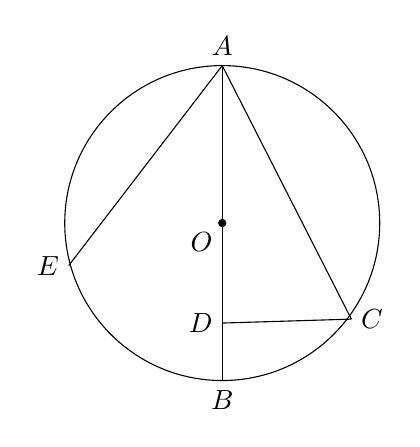
\begin{tikzpicture}
\coordinate (O) at (0,0);
\coordinate (A) at (0,2);
\coordinate (B) at (0,-2);
\coordinate (D) at (0,-1.27);
\coordinate (C) at (1.64,-1.22);
\coordinate (E) at (-1.95,-0.54);

\draw (O) circle (2);
\draw (A) -- (E);
\draw (A) -- (C);
\draw (A) -- (B);
\draw (D) -- (C);

\fill (O) circle (1.5pt);

\node[above] at (A) {$A$};
\node[below] at (B) {$B$};
\node[right] at (C) {$C$};
\node[left] at (D) {$D$};
\node[left] at (E) {$E$};
\node[below left] at (O) {$O$};
\end{tikzpicture}
\end{document}
